\input{mmd-article-header}
\def\mytitle{Chapter 2 -- DLS Studies and Protocol Optimization}
\input{mmd-article-begin-doc}
\def\bibliocommand{\bibliography{theis.bib}}
\chapter{Characterization of 5 kDa PEG-SH}
\label{characterizationof5kdapeg-sh}

In the spring of 2011, several experiments were performed to characterize the 5 kDa PEG-SH (PS), which is used to provide protection to the Au nanospheres. The PS was characterized in three ways: a titration, a time study, and a protection study. These demonstrated that a number concentration of $50,\,000$ PS molecules per Au nanosphere, after 24 hours of incubation, should provide complete long-term protection to the Au nanospheres in a salt-rich environment.

\section{Titration Study}
\label{titrationstudy}

A titration curve was made by adding 5 kDa PS to 90 nm gold nanospheres (R=53 nm) in varying concentrations, from 1000 PS per nanosphere to $10^7$ PS per nanosphere. The hydrodynamic radii of these PEGylated nanospheres were then measured using the Dynamic Light Scattering (DLS) instrument, taking 15 30-second acquisitions of each solution and discarding the first three to account for temperature acclimation. This procedure was performed three separate times; a plot of the results is shown in \autoref{kdapegshnew}.

\begin{figure}[htbp]
\centering
\includegraphics[keepaspectratio,width=\textwidth,height=0.75\textheight]{../../../Archived.Work/HMC.11.SP/Research/5kdaPEGSHnew.pdf}
\caption{Plot of hydrodynamic radius of Au nanospheres with at various concentrations less than 30 minutes after addition of PS.}
\label{kdapegshnew}
\end{figure}



This plot shows the behavior of a rapid rise followed by a plateau that is expected of a species forming a monolayer on a surface. The plateau begins at approximately $5\times10^4$ PS molecules per nanosphere with R=60--61 nm, and has an elbow at around $10^4$ PS per nanosphere.

\section{Time Study}
\label{timestudy}

The same samples used in the titration study were measured again after 48--72 hours of incubation, producing the radii shown in \autoref{kdapegshtime}.

\begin{figure}[htbp]
\centering
\includegraphics[keepaspectratio,width=\textwidth,height=0.75\textheight]{../../../Archived.Work/HMC.11.SP/Research/5kdaPEGSHtime.pdf}
\caption{Plot of hydrodynamic radius of Au nanospheres with at various concentrations 48--72 hours after addition of PS.}
\label{kdapegshtime}
\end{figure}



The plateau in this graph is much sharper than in \autoref{kdapegshnew}, indicating that van der Waals forces and thiol bonding processes are in competition, with van der Waals binding dominating immediately after addition, but the lower-energy thiol bonds dominating after incubation time. This leads to the increased radius of the lower-radius samples and the decreased radius of the higher-radius samples. However, the plateau region still has R=60--61 nm, as a second indication of a monolayer. Clearly, it is essential that PEG-SH be allowed to incubate with spheres to allow for the PEG-SH binding to reach equilibrium.

\section{Protection Study}
\label{protectionstudy}

As mentioned above, the main reason for using 5 kDa PEG-SH is to prevent the Au nanospheres from conglomeration. The Au nanosphere solution includes a negatively charged capping agent that makes the spheres repel each other; when the solution is buffered at pH \ensuremath{\sim}7.5 to prevent antibodies from denaturing during the full immunogold procedure, positive ions are introduced into the solution that neutralize the capping agents, causing the gold nanospheres to agglomerate. Theoretically, PEG-SH would prevent this from happening, but 1 kDa PEG-SH does not, as shown in \autoref{protection1kda}.

\begin{figure}[htbp]
\centering
\includegraphics[keepaspectratio,width=4in,height=0.75\textheight]{../../../Archived.Work/HMC.11.SP/Research/Protection1kDa.pdf}
\caption{Histogram of radii of acquisitions of 300k 1 kDa PS\slash Au with and without PBS from Summer 2010. The distribution is noticeably shifted to the right and flattened after the addition of PBS. Data taken by Ellis and Hoidn~\citep{hoidnellis}.}
\label{protection1kda}
\end{figure}



Therefore, the protection capabilities of 5 kDa PS were tested by adding PEG-SH to the Au nanospheres in various concentrations, then mixing those solutions in equal volumes with commercial phosphate buffered saline. The spheres were allowed to incubate for at least 30 minutes with the PBS, then measured in the DLS. Selected results from those measurements are shown in \autoref{protection}.

\begin{figure}[htbp]
\centering
\includegraphics[keepaspectratio,width=4in,height=0.75\textheight]{../../../Archived.Work/HMC.11.SP/Research/protection.pdf}
\caption{Stacked histograms of differing concentrations of Au-PS with and without PBS. The naked gold is significantly broader than any of the other distributions.}
\label{protection}
\end{figure}



For all but the naked gold, almost all acquisitions are within 3 nm of the mean; this is also true of the 300k PS\slash Au without PBS from Summer 2010. However, with just 10k 5 kDa PS\slash Au, the width of the distribution barely widens when PBS is added--a stark contrast to the addition of PBS to 300k 1 kDa PS\slash Au. Furthermore, there was a \ensuremath{\sim}15 nm increase in average radius between the 1 kDa PS spheres with and without PBS. In the case of the 10k 5 kDa PS\slash Au, the difference in average radius was negligible: 0.09 nm.

From observing the lack of change in both average radius and the change in radial distribution when using the 5 kDa PEG-SH, it is clear that the 5 kDa PEG-SH fully protects the Au nanospheres against capping agent neutralization. There is, however, a noticeable difference between the 10k and 300k PS\slash Au samples; the 300k is slightly narrower, indicating that it offers slightly more protection, consistent with the 300k PS\slash Au solution being on the plateau while the 10k PS\slash Au is still on the rising part of the titration curve.

\chapter{Results of the Complete Binding Protocol}
\label{resultsofthecompletebindingprotocol}

Several fully labeled and protected nanosphere samples were created during the '11--'12 year. The protocol used was adapted from Oliver Hoidn and Perry Ellis's report~\citep{hoidnellis}, using 2,000 antibodies per Au nanosphere and the curve-elbow value 10,000 PEG-SH molecules per Au nanosphere. Detailed documentation of the protocol can be found in \autoref{a:protocol}.

The progress of the protocol was monitored by a DLS radius measurement at five or six stages:

\begin{enumerate}
\item Immediately after the addition of the OPAb

\item 24 hours after the addition of the OPAb

\item Immediately after the addition of the PEG-SH

\item 24 hours after the addition of the PEG-SH

\item After dilution with equal parts PBS, to check for protection

\item (For most but not all samples) 48 hours after the addition of PEG-SH

\end{enumerate}

The results of these measurements are shown in \autoref{fullprotocol}. The data shows an immediate increase of 6--8 nm upon the addition of the OPAb, followed by slight ($<$0.1 nm) gains after 24 hours of incubation. AP124F is an IgG antibody and has dimensions of approximately $14.5\mathrm{\,nm}\times8.5\mathrm{\,nm}\times4.0\mathrm{\,nm}$~\citep{antibodylength} as shown in \autoref{iggstructure};
since the NHS replacement can occur on any lysine or N terminus (of which there are several), a 6--8 nm increase in radius is reasonable when all spatial orientations are taken into account.

\begin{figure}[htbp]
\centering
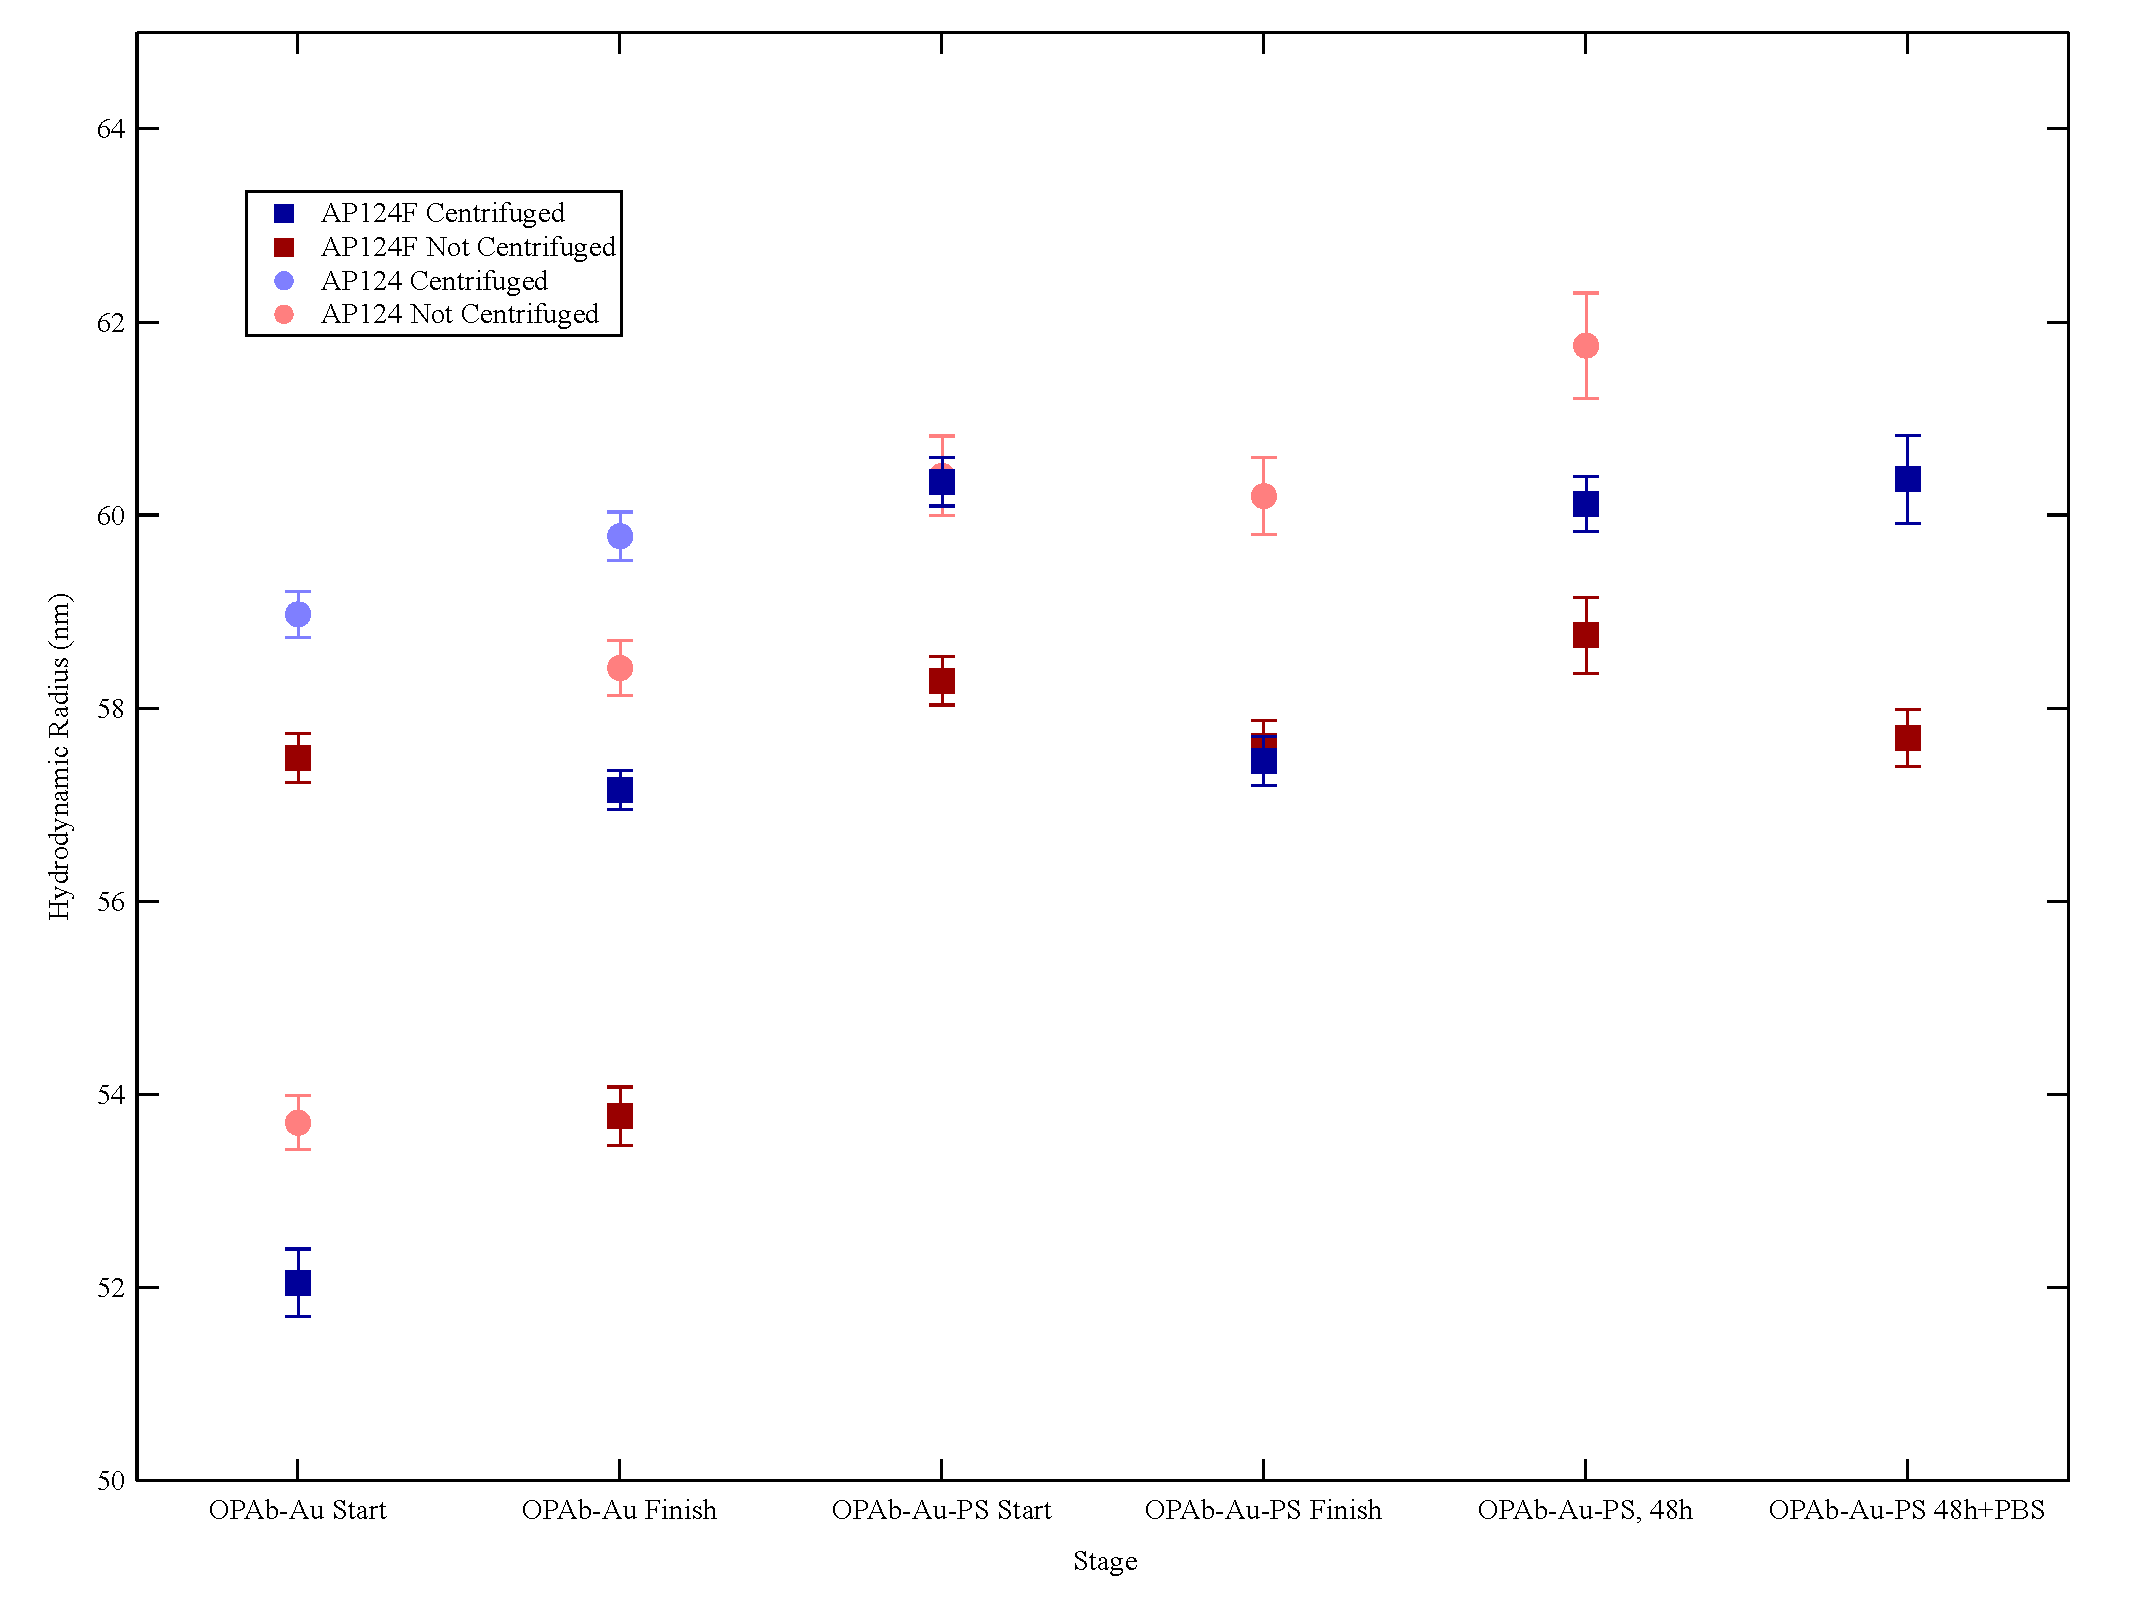
\includegraphics[keepaspectratio,width=\textwidth,height=0.75\textheight]{2011DecPEGylation.pdf}
\caption{Plot of hydrodynamic radii of multiple solutions at each step in the protocol. NOTE: PLACEHOLDER UNTIL I COLLATE ALL THE DATA.}
\label{fullprotocol}
\end{figure}

\begin{figure}[htbp]
\centering
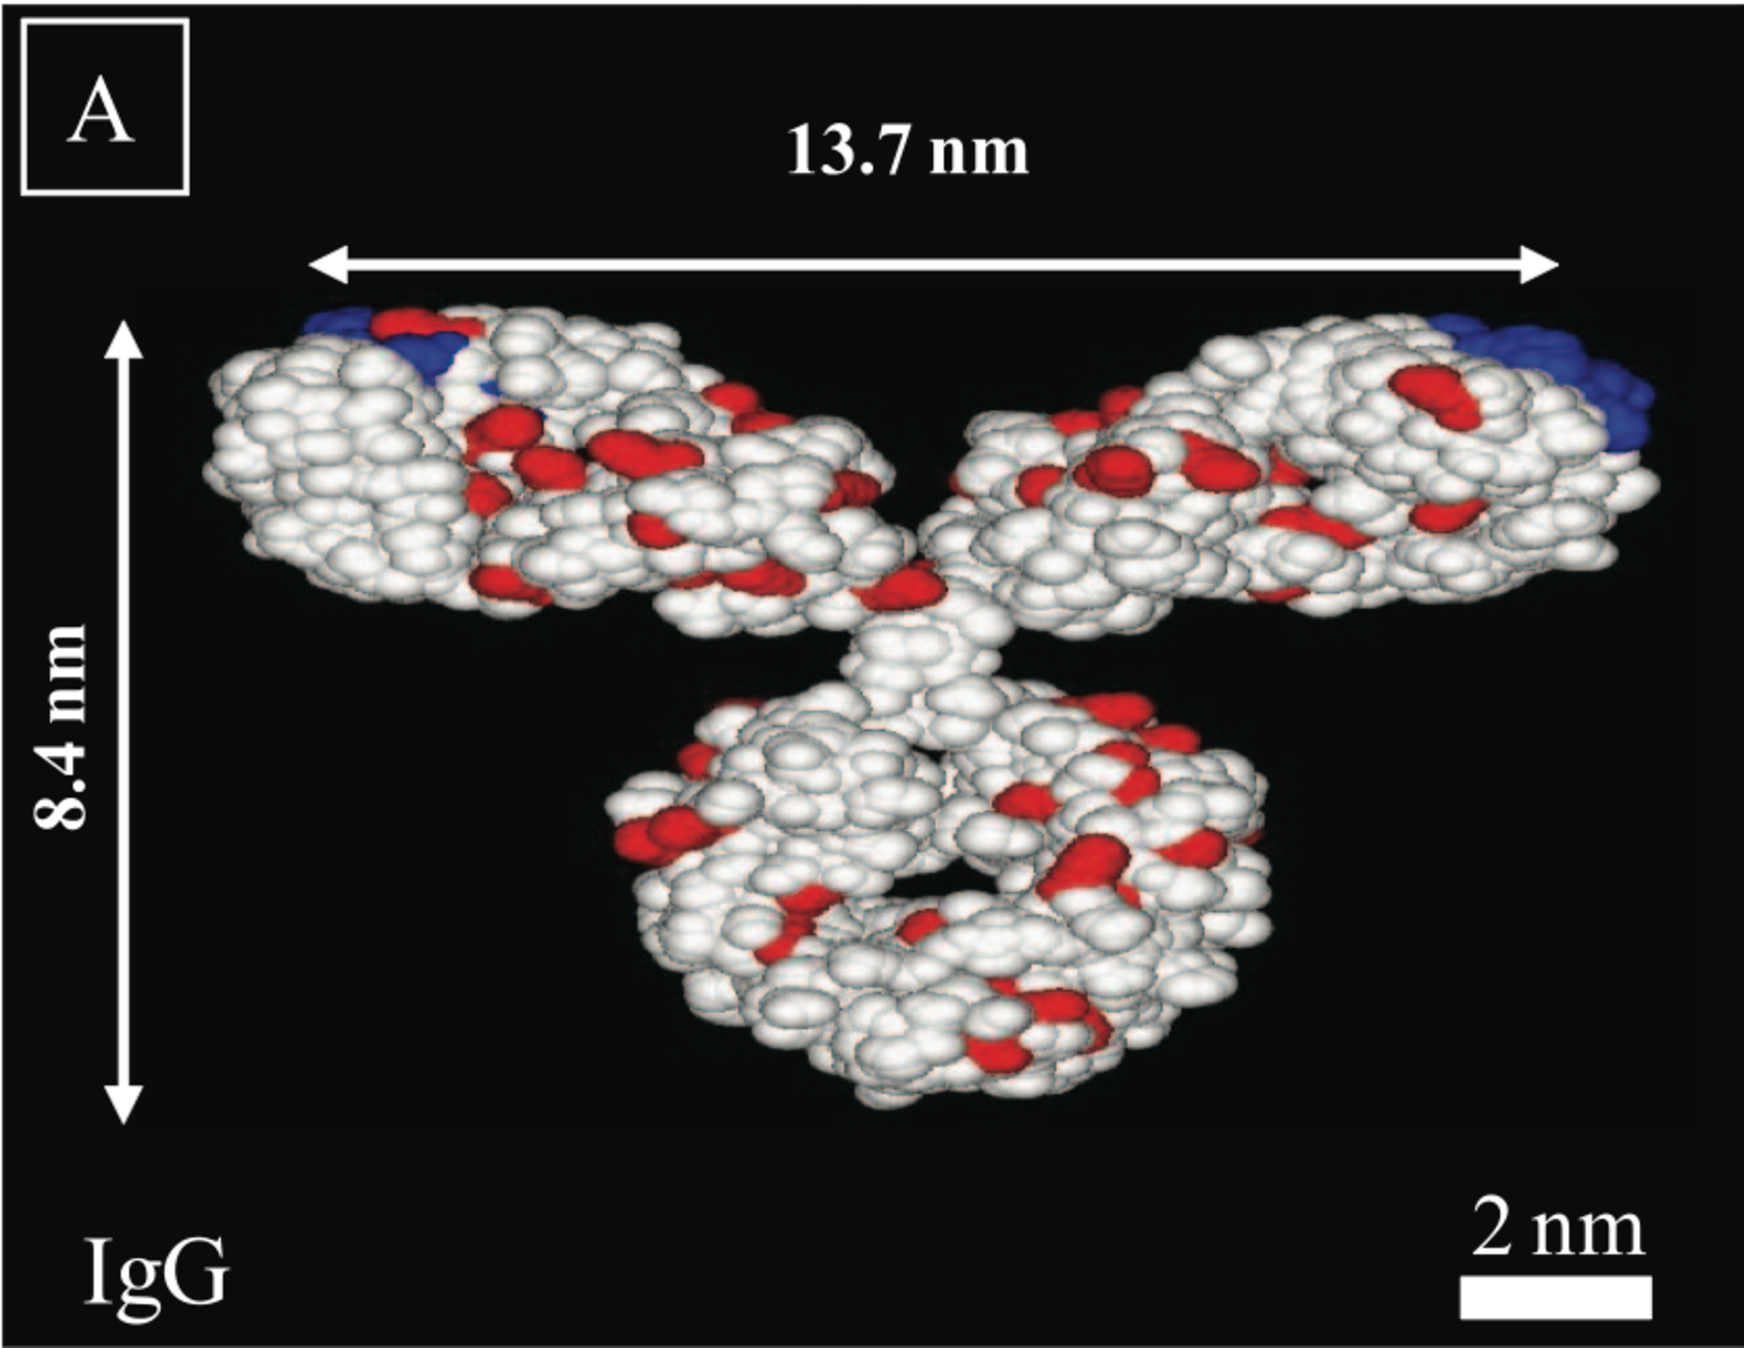
\includegraphics[keepaspectratio,width=3in,height=0.75\textheight]{iggstructure.pdf}
\caption{Structure dimensions of an IgG antibody. From ~\citep{antibodylength}.}
\label{iggstructure}
\end{figure}

An OPAb conjugate should have a volume of
\[V=V_{\mathrm{PEG}}+V_{\mathrm{Ab}}=\frac{2.1\mathrm{kDa}}{1.11\frac{\mathrm g}{\mathrm cm^3}}+\frac{160\mathrm{kDa}}{1.35\frac{\mathrm g}{\mathrm cm^3}}=200\,\mathrm{nm}^3\]
Examining the hydrodynamic volume change after the addition of PEG-SH, this corresponds to
\[\frac{4}{3}\pi[(58\mathrm{\,nm})^3-(51.5\mathrm{\,nm})^3]/200\frac{\mathrm{nm}^3}{OPAb}=1230\mathrm{\ OPAb}\]
However, this is likely an under-estimate, as the 1.35 $\mathrm{\frac{g}{cm^3}}$ density is for the crystalline state of protein~\citep{proteindensity}; the actual effective volume of the OPAb in solution is likely larger. Further uncertainty is introduced by the complexity of the diffusion of an Au nanosphere with over 1000 OPAb molecules attached to it. Therefore, this calculation serves primarily as an order-of-magnitude check; in that sense, 1230 OPAb\slash Au compares quite favorably to the 2000 OPAb\slash Au in solution.

\input{mmd-memoir-footer}

\end{document}
